%%%%%%%%%%%%%%%%%%%%%%%%%%%%%%%%%%%
%This is the LaTeX ARTICLE template for RSC journals
%Copyright The Royal Society of Chemistry 2016
%%%%%%%%%%%%%%%%%%%%%%%%%%%%%%%%%%%


\documentclass[twoside,twocolumn,9pt]{article}
\usepackage{extsizes}
\usepackage[super,sort&compress,comma]{natbib} 
\usepackage[version=3]{mhchem}
\usepackage[left=1.5cm, right=1.5cm, top=1.785cm, bottom=2.0cm]{geometry}
\usepackage{balance}
\usepackage{mathptmx}
\usepackage{sectsty}
\usepackage{graphicx} 
\usepackage{lastpage}
\usepackage[format=plain,justification=justified,singlelinecheck=false,font={stretch=1.125,small,sf},labelfont=bf,labelsep=space]{caption}
\usepackage{float}
\usepackage{fancyhdr}
\usepackage{fnpos}
%\addto{\captionsenglish}{%
%  \renewcommand{\refname}{Notes and references}
%}
\usepackage{array}
\usepackage{droidsans}
\usepackage{charter}
\usepackage[T1]{fontenc}
\usepackage[usenames,dvipsnames]{xcolor}
\usepackage{setspace}
\usepackage[compact]{titlesec}
\usepackage{hyperref}
\usepackage{array,longtable}
\usepackage{supertabular,booktabs}
%%%%%%%%%%%%%%
\usepackage[OT2, T1]{fontenc}
\usepackage[english]{babel}
\usepackage[utf8]{inputenc}
\usepackage[T2A]{fontenc}
%\usepackage[russian, english]{babel}
%\usepackage[T2A,T1]{fontenc}
%\usepackage[utf8]{inputenc}
%\usepackage[russian,english]{babel}
%%%Please don't disable any packages in the preamble, as this may cause the template to display incorrectly.%%%


\usepackage{epstopdf}%This line makes .eps figures into .pdf - please comment out if not required.

\definecolor{cream}{RGB}{222,217,201}

%%%%%%%%%%%%%%%%%%%%%%
\usepackage{changes}
\usepackage{lipsum}% <- For dummy text
\definechangesauthor[name={Per cusse}, color=orange]{per}
\setremarkmarkup{(#2)}

\usepackage{soul}
\begin{document}

\pagestyle{fancy}
\thispagestyle{plain}
\fancypagestyle{plain}{
%%%HEADER%%%
\renewcommand{\headrulewidth}{0pt}
}
%%%END OF HEADER%%%

%%%PAGE SETUP - Please do not change any commands within this section%%%
\makeFNbottom
\makeatletter
\renewcommand\LARGE{\@setfontsize\LARGE{15pt}{17}}
\renewcommand\Large{\@setfontsize\Large{12pt}{14}}
\renewcommand\large{\@setfontsize\large{10pt}{12}}
\renewcommand\footnotesize{\@setfontsize\footnotesize{7pt}{10}}
\makeatother

\renewcommand{\thefootnote}{\fnsymbol{footnote}}
\renewcommand\footnoterule{\vspace*{1pt}% 
\color{cream}\hrule width 3.5in height 0.4pt \color{black}\vspace*{5pt}} 
\setcounter{secnumdepth}{5}

\makeatletter 
\renewcommand\@biblabel[1]{#1}            
\renewcommand\@makefntext[1]% 
{\noindent\makebox[0pt][r]{\@thefnmark\,}#1}
\makeatother 
\renewcommand{\figurename}{\small{Fig.}~}
\sectionfont{\sffamily\Large}
\subsectionfont{\normalsize}
\subsubsectionfont{\bf}
\setstretch{1.125} %In particular, please do not alter this line.
\setlength{\skip\footins}{0.8cm}
\setlength{\footnotesep}{0.25cm}
\setlength{\jot}{10pt}
\titlespacing*{\section}{0pt}{4pt}{4pt}
\titlespacing*{\subsection}{0pt}{15pt}{1pt}
%%%END OF PAGE SETUP%%%

%%%FOOTER%%%
\fancyfoot{}
\fancyfoot[LO,RE]{\vspace{-7.1pt}
\includegraphics[height=9pt]{head_foot/LF}}
\fancyfoot[CO]{\vspace{-7.1pt}\hspace{13.2cm}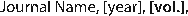
\includegraphics{head_foot/RF}}
\fancyfoot[CE]{\vspace{-7.2pt}\hspace{-14.2cm}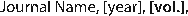
\includegraphics{head_foot/RF}}
\fancyfoot[RO]{\footnotesize{\sffamily{1--\pageref{LastPage} ~\textbar  \hspace{2pt}\thepage}}}
\fancyfoot[LE]{\footnotesize{\sffamily{\thepage~\textbar\hspace{3.45cm} 1--\pageref{LastPage}}}}
\fancyhead{}
\renewcommand{\headrulewidth}{0pt} 
\renewcommand{\footrulewidth}{0pt}
\setlength{\arrayrulewidth}{1pt}
\setlength{\columnsep}{6.5mm}
\setlength\bibsep{1pt}
%%%END OF FOOTER%%%

%%%FIGURE SETUP - please do not change any commands within this section%%%
\makeatletter 
\newlength{\figrulesep} 
\setlength{\figrulesep}{0.5\textfloatsep} 

\newcommand{\topfigrule}{\vspace*{-1pt}% 
\noindent{\color{cream}\rule[-\figrulesep]{\columnwidth}{1.5pt}} }

\newcommand{\botfigrule}{\vspace*{-2pt}% 
\noindent{\color{cream}\rule[\figrulesep]{\columnwidth}{1.5pt}} }

\newcommand{\dblfigrule}{\vspace*{-1pt}% 
\noindent{\color{cream}\rule[-\figrulesep]{\textwidth}{1.5pt}} }

\makeatother
%%%END OF FIGURE SETUP%%%

%%%TITLE, AUTHORS AND ABSTRACT%%%
\twocolumn[
  \begin{@twocolumnfalse}
{
\includegraphics[height=30pt]{head_foot/journal_name}\hfill\raisebox{0pt}[0pt][0pt]{
\includegraphics[height=55pt]{head_foot/RSC_LOGO_CMYK}}\\[1ex]

\includegraphics[width=18.5cm]{head_foot/header_bar}}\par
\vspace{1em}
\sffamily
\begin{tabular}{m{4.5cm} p{13.5cm} }


\includegraphics{head_foot/DOI} & \noindent\LARGE{\textbf{Phase stability in nickel phosphides at high pressures %$^\dag$
}} \\%Article title goes here instead of the text "This is the title"
\vspace{0.3cm} & \vspace{0.3cm} \\

 & \noindent\large{Talgat M.~Inerbaev,$^{\ast}$\textit{$^{ab}$} Nursultan Sagatov,\textit{$^{ac}$}, Dinara Sagatova,\textit{$^{ac}$} Pavel N.  Gavryushkin,\textit{$^{ac}$} 
 
 Abdirash T. Akilbekov,\textit{$^{b}$} and Konstantin D. Litasov\textit{$^{de}$}} \\%Author names go here instead of "Full name", etc.

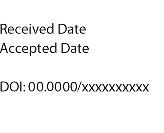
\includegraphics{head_foot/dates} & \noindent\normalsize{
%
Phosphorus – one of the light elements of the Earth's core and planets.
High-pressure behaviour of phosphorus compounds with nickel and iron attracts considerable attention due to their findings in meteorites and mantle xenolites {\color{red}(Константин, поправь меня, если я не прав)}
In the present work, with modern methods of crystal structure prediction we investigate structures and stability of compounds in Ni-P system at pressures of 100-400 GPa.
As the result the series of (Ni,P) solid solutions, presents by compounds Ni$_{14}$P, Ni$_{12}$P, Ni$_{10}$P, Ni$_8$P, Ni$_7$P, Ni$_5$P, and Ni$_3$P, is revealed.
Phosphorus show sufficient solubility in $fcc$ structure of Ni, and up to 25 mol.\% of this element can be dissolved at low temperatures.
Based on the comparison of compounds in Ni-P and Fe-P systems we suggest, that at high pressures Ni facilitates phosphorus dissolution in closed-packed structure of $d$-metals, and dissolution of P in (Ni,P) alloy will be higher, than in pure Fe.
For the Ni$_3$P compound, a new high-pressure phase with $Cmca$ symmetry is revealed. 
This structure can be described as deformed $fcc$ packing and also belongs to the series of (Ni,P) solid solutions.
The transition from the low-pressure phase of Ni$_3$P-$I\bar{4}$ to the $Cmca$ phase occurs at a pressure of 62~GPa, regardless of the external temperature. 
Ni$_2$P is stabilised at pressure above 200 GPa in the form of allabogdanite structure.
The transition from barringerite to allabogdanite is predicted to occur in the range of 78--88~GPa at temperatures 0-2000~K. 


%
} \\%The abstract goes here instead of the text "The abstract should be..."

\end{tabular}

 \end{@twocolumnfalse} \vspace{0.6cm}

]
%%%END OF TITLE, AUTHORS AND ABSTRACT%%%

%%%FONT SETUP - please do not change any commands within this section
\renewcommand*\rmdefault{bch}\normalfont\upshape
\rmfamily
\section*{}
\vspace{-1cm}


%%%FOOTNOTES%%%

\footnotetext{\textit{$^{a}$~Sobolev Institute of Geology and Mineralogy, Siberian Branch of the Russian Academy of Sciences, Novosibirsk, 630090 Russia. E-mail: inerbaevtm@igm.nsc.ru}}
\footnotetext{\textit{$^{b}$~L. N. Gumilyov Eurasian National University, Nur-Sultan, 010008 Kazakhstan.}} 
\footnotetext{\textit{$^{c}$~Novosibirsk State University, Novosibirsk, 630090 Russia.}}
\footnotetext{\textit{$^{d}$~Vereshchagin Institute for High Pressure Physics, Russian Academy of Sciences, Moscow, 108840, Russia.}}
\footnotetext{\textit{$^{e}$~Fersman Mineralogical Museum Russian Academy of Sciences, Moscow, Russia.}}
%Please use \dag to cite the ESI in the main text of the article.
%If you article does not have ESI please remove the the \dag symbol from the title and the footnotetext below.
%\footnotetext{\dag~Electronic supplementary information (ESI) available: Method of quasi-harmonic approximation, phonon dispersion curves, structures predicted by USPEX and AIRSS method. See DOI: 00.0000/00000000.} 
%additional addresses can be cited as above using the lower-case letters, c, d, e... If all authors are from the same address, no letter is required

%\footnotetext{\ddag~Additional footnotes to the title and authors can be included \textit{e.g.}\ `Present address:' or `These authors contributed equally to this work' as above using the symbols: \ddag, \textsection, and \P. Please place the appropriate symbol next to the author's name and include a \texttt{\textbackslash footnotetext} entry in the the correct place in the list.}


%%%END OF FOOTNOTES%%%

%%%MAIN TEXT%%%%
%The main text of the article\cite{Mena2000} should appear here.
\section{Introduction}

Phosphides play a significant role in the mineralogy of iron meteorites as the components of the ternary Fe-Ni-P system. 
Although being rare, accessory minerals  with  composition  (Fe,Ni)$_x$P, they give important information about phosphorus geochemistry on the early stages of the universe formation. \cite{Skala2005, skala_m-2003, Buseck1969, Britvin-2002, Pratesi-2006, reed_1968, Britvin2019-SciRep, Britvin2019-PCM-Fe2P, Britvin2019-murashkoite-MP-FeP, Britvin2020-Halamishite}
The occurrence  of  these  minerals  in  meteoritic  samples  is  believed  to originate either from the equilibrium condensation of protoplanetary materials  taking  place in the solar nebulae  or  from  crystallization processes  in  the  cores  of  parent  bodies. 
%From the analysis of iron meteorites and the observation of Earth's moment of inertia, it is known that the primary constituent of Earth's inner core is an iron-nickel alloy~\cite{Birch-1992} with Fe/Ni$\sim$16.~\cite{ALLEGRE-1995-515,MCDONOUGH-1995-223}
%At the same time, geochemical and geophysical studies show that light elements (i.e. hydrogen, oxygen, carbon, sulfur, phosphorus and silicon) play important roles in the Earth's core.~\cite{POIRIER-1994-319,Cote-2008-GRL}

%Phosphorus is one of the elements believed to be present in the Earth's core. \cite{Stewart-2007-GRL}
%Its content of the Earth's core was estimated to be <1~wt\%.~\cite{ALLEGRE-1995-515,MCDONOUGH-1995-223,McDonough2004book}
%High concentrations of phosphorus (up to 4 wt\%) are able to dissolve into iron at high pressures over a wide temperature range.\cite{Stewart-2007-GRL}


Iron-rich end-members of Fe--P system were intensively studied using both experimental and theoretical techniques. 
So far, most of the high-pressure investigations on iron phosphides have been restricted on Fe$_4$P,~\cite{Wu-2011-GRL} Fe$_3$P,~\cite{Scott-2007-GRL} Fe$_2$P~\cite{Dera-2008-GRL, Wu_2010-JPCM}, and FeP.~\cite{Gu-2011-FeP-EPS}
Several structural and magnetic phase transitions have been revealed as the result. 
Dera et al. observed that on heating at 8 GPa phase of Fe$_2$P transforms to a high-pressure modification, which could be quenched to ambient conditions.~\cite{Dera-2008-GRL} 
Theoretical modelling demonstrates that the stable phase of Fe$_2$P should be the $Pnma$ with the lowest total energy in the low pressure region, and the $P\bar{6}2m$ and $Pnma$ phases would transform to the $P\bar{3}m$ phase with larger coordination number of iron at 125~GPa and 153~GPa, respectively.~\cite{Wu_2010-JPCM} 
Theoretical studies have shown that Fe$_3$P could decompose into Fe$_2$P and Fe$_4$P at pressures higher than 214~GPa ~\cite{Zhao-2017-RSC-Adv}, and Fe$_3$P and Fe would react with formation of Fe$_4$P at $\sim$100 GPa.~\cite{Wu-2011-GRL} 
Fe$_3$P exhibits a structural phase transition from $I4$ to $P4/mnc$ at 64~GPa and 1600~K accompanied with an electronic state transition from high-spin to low-spin at around 20-40~GPa.~\cite{GU2014-EPSL, Gu-2016-AmMiner-Fe3P}
Upon compression, Fe$_4$P undergoes transition from ferromagnetic to nonmagnetic state at 80~GPa.\cite{Wu-2011-GRL}
Britvin et al. reported two new structures of FeP ($Pnma$) and FeP$_2$ ($Pnnm$), found in the pyrometamorphic rocks.  \cite {Britvin2019-PCM-Fe2P,Britvin2019-murashkoite-MP-FeP}

\begin{table*}[t]
\small
  \caption{\ Structural data for the found phases of Ni--P system 
{\color{red}–(1) Здесь необходимо привести данные предсказанного аллабогданита-Ni$_2$P, чтобы желающие могли убедиться что это действительно аллабогданит. Параметры ячейки могут пригодиться экспериментаторам для расшифровки дифрактограмм. Вообщем привести стоит.
– (2) Параметры ячейки лучше округлить до тысячных, четвёртая цифра абсолютно не значима. Координаты атомов – до десятитысячных (именно так делает большинство авторов, например К. Пикард, лично я бы всё до тысячных округлял))
– (3) С помощью функции multirow можно сделать, чтобы названия Phase, Pressure и пр., были в центре ячейки
– (4) В ячейке Lattice parameters в скобках указано (\AA, degree), а потом в таблице снова стоят \AA 
– (5) Структурные данные лучше приводить для наиболее низкого давления (в поле стабильности, конечно), потому что при 400 ГПа эксперименты никто ставить не будет. И данные лучше приводить для одного и того же давления, чтобы можно было сравнить объемы. Вообщем, все твёрдые растворы лучше привести на 100 ГПа.}
}
  \label{tbl:new_phases}
  \begin{tabular*}{\textwidth}{@{\extracolsep{\fill}}llllllllll}
    \hline
    \multicolumn{6}{l}{} & \multicolumn{4}{c}{Atomic coordinates}\\\cline{7-10}
%     &  &  &  &  &   &  & & & \\\cline{7-10}
    Phase & Pressure (GPa) & Space group & \multicolumn{3}{c}{Lattice parameters (\AA, degree)}  & Atom & $x$ & $y$ & $z$\\
    \midrule
    Ni$_{14}$P & 400 & $C2/m$ (\#12) & $a$=6.8686\AA    & $b$=6.2097\AA   & $c$=5.0749\AA    & Ni1 & 0.00000 & 0.16860 & 0.00000 \\
               &     &               & $\alpha$=90      & $\beta$=119.559 & $\gamma$=90      & Ni2 & 0.09850 & 0.00000 & 0.39699 \\    
               &     &               &                  &                 &                  & Ni3 & 0.30065 & 0.00000 & 0.19837 \\
               &     &               &                  &                 &                  & Ni4 & 0.70280 & 0.33474 & 0.80023 \\
               &     &               &                  &                 &                  & Ni5 & 0.59887 & 0.16587 & 0.39807 \\
               &     &               &                  &                 &                  & P1  & 0.00000 & 0.50000 & 0.00000 \\
%%%%%%%%%%%%%%%%%%%%%%%%%%%%%%%%%%%%%%%%%%%%%%%%%%%%%%%%%%%%%%%%%%%%%%%%%%%%%%%%%%%%%%%%%%%%%%%%%%%%%%%%%%%%%%%%%%%%%%%%%%%%%%%%%%
\midrule
    Ni$_{12}$P & 400 & $R\bar3$(\#148)    & $a$=7.4609\AA    & $b$=7.4609\AA   & $c$=5.0755\AA    & Ni1 & 0.53902  & 0.38422 & 0.00134 \\
               &     &               & $\alpha$=90.00   & $\beta$=90.00 & $\gamma$=120       & Ni2 & -0.02851 & 0.40876 & 0.33153 \\
               &     &               &                  &                 &                  & P1  & 0.00000  & 0.00000 & 0.00000 \\
%%%%%%%%%%%%%%%%%%%%%%%%%%%%%%%%%%%%%%%%%%%%%%%%%%%%%%%%%%%%%%%%%%%%%%%%%%%%%%%%%%%%%%%%%%%%%%%%%%%%%%%%%%%%%%%%%%%%%%%%%%%%%%%%%%
\midrule
    Ni$_{10}$P & 300 & $P\bar{1}$ (\#2)     & $a$=3.6654\AA    & $b$=4.7295\AA   & $c$=4.7339\AA    & Ni1 & 0.04502 & 0.41007 & 0.18032 \\
               &     &               & $\alpha$=107.482 & $\beta$=104.937 & $\gamma$=97.456  & Ni2 & 0.59015 & 0.31912 & 0.35915 \\
               &     &               &                  &                 &                  & Ni3 & 0.13716 & 0.22851 & 0.54678 \\
               &     &               &                  &                 &                  & Ni4 & 0.22672 & 0.04944 & -0.09103\\
               &     &               &                  &                 &                  & Ni5 & 0.67759 & 0.13805 & 0.72806 \\
               &     &               &                  &                 &                  & P1  & 0.50000 & 0.50000 & 0.00000 \\
\midrule
%%%%%%%%%%%%%%%%%%%%%%%%%%%%%%%%%%%%%%%%%%%%%%%%%%%%%%%%%%%%%%%%%%%%%%%%%%%%%%%%%%%%%%%%%%%%%%%%%%%%%%%%%%%%%%%%%%%%%%%%%%%%%%%%%%
    Ni$_{8}$P  & 200 & $P\bar{1}$ (\#2)     & $a$=3.7669\AA    & $b$=3.7719\AA   & $c$=4.8694\AA    & Ni1 & 0.22148 & 0.11048 & 0.56082 \\
               &     &               & $\alpha$=75.00 & $\beta$=82.569 & $\gamma$=80.481     & Ni2 & 0.67093 & 0.33311 & 0.66740 \\
               &     &               &                  &                 &                  & Ni3 & 0.44401 & 0.21845 & 0.11085 \\
               &     &               &                  &                 &                  & Ni4 & 0.11116 & 0.55650 & 0.78047 \\
               &     &               &                  &                 &                  & P1  & 0.00000 & 0.00000 & 0.00000 \\
\midrule
%%%%%%%%%%%%%%%%%%%%%%%%%%%%%%%%%%%%%%%%%%%%%%%%%%%%%%%%%%%%%%%%%%%%%%%%%%%%%%%%%%%%%%%%%%%%%%%%%%%%%%%%%%%%%%%%%%%%%%%%%%%%%%%%%%
    Ni$_{7}$P  & 100 & $P\bar{1}$ (\#2)     & $a$=3.7553\AA    & $b$=3.7772\AA   & $c$=4.3925\AA    & Ni1 &  0.50201 & 0.00029 & 0.24766 \\
               &     &               & $\alpha$=73.032 & $\beta$=89.980 & $\gamma$=79.849    & Ni2 &  0.00000 & 0.00000 & 0.50000 \\
               &     &               &                  &                 &                  & Ni3 &  0.75389 & 0.49840 & 0.12435 \\
               &     &               &                  &                 &                  & Ni4 &  0.24895 & 0.50693 & 0.37130 \\
               &     &               &                  &                 &                  & P1  &  0.00000 & 0.00000 & 0.00000 \\
%%%%%%%%%%%%%%%%%%%%%%%%%%%%%%%%%%%%%%%%%%%%%%%%%%%%%%%%%%%%%%%%%%%%%%%%%%%%%%%%%%%%%%%%%%%%%%%%%%%%%%%%%%%%%%%%%%%%%%%%%%%%%%%%%%%%%%%%%%%%
\midrule
    Ni$_{5}$P  & 200 & $P6_3/mcm$ (\#193)  & $a$=3.7732\AA    & $b$=3.7732\AA   & $c$=7.0786\AA    & Ni1 & 0.33333   &  0.66667  &   0.00000  \\
               &     &                    & $\alpha$=90.00   & $\beta$=90.00 & $\gamma$=120       & Ni2 & 0.67096   &  0.00000  &   0.25000  \\
               &     &                    &                  &                 &                  & P1 &  0.00000    & 0.00000   &  0.00000  \\
\midrule
%%%%%%%%%%%%%%%%%%%%%%%%%%%%%%%%%%%%%%%%%%%%%%%%%%%%%%%%%%%%%%%%%%%%%%%%%%%%%%%%%%%%%%%%%%%%%%%%%%%%%%%%%%%%%%%%%%%%%%%%%%%%%%%%%%
    Ni$_{3}$P  & 100 & $Cmca$ (\#64) & $a$=13.1666\AA   & $b$=4.4854\AA   & $c$=4.4851\AA    & Ni1 & 0.38137   &  0.00000  &   0.00000  \\
               &     &               & $\alpha$=90.00   & $\beta$=90.00   & $\gamma$=90.00   & Ni2 & 0.00000   &  0.18176  &   0.81801  \\
               &     &               &                  &                 &                  & Ni3 & 0.25000   &  0.74729  &   0.25000  \\   
               &     &               &                  &                 &                  & P1 &  0.13651    & 0.00000   &  0.00000  \\
\hline
               %    \midrule
  \end{tabular*}
\end{table*}




%{\textbf{He 2018}}
Alloying effect of Ni on physical properties and structure of Fe and it's alloys with light elements is also of geological interest, as according to geochemical assesment Earth's core could contain up to 10mol\% of Ni \cite{} {\color{red}(Уточнить и поставить ссылку на Чёрную Книжку (?))}.
Addition of nickel to iron phosphides affect the structure and phase stability. 
The example of Fe$_2$P shows, that even a small addition of Ni and Co stabilise the structure of alabogdanite against XXX ~\cite{Britvin-2002, Buseck1969, Nisar-2010-EPSL}, and also slightly increases the  bulk modulus of the allabogdanite phase.~\cite{Nisar-2010-EPSL} 
А может здесь сослаться на нашу статью по алабогданиту (Bekker, Sagatov et al., 2020)?
The incorporation of Ni in nonmagnetic Fe$_4$P results in reduction of the compressional and shear wave velocities enhancing their anisotropy.\cite{Wu-2011-GRL}

%\textbf{Litasov2019}
There are numerous phases were revealed in Ni--P system at ambient pressure. 
Among them are Ni$_3$P, Ni$_8$P$_3$, Ni$_{12}$P$_5$ , Ni$_2$P, Ni$_5$P$_4$, NiP, NiP$_2$, and NiP$_3$. 
Вижу здесь NiP3, Ni5P4, Ni$_{12}$P$_5$. Возникает вопрос, а почему мы их на выпуклую оболочку не нанесли? Ni8P3 и NiP2 нанесли, а эти нет? Какой принцип для выбора фаз? По-хорошему следовало бы для всех этих составов провести предсказания, как мы это делали с гидридами. В Методику нужно обязательно добавить, что какие-то фазы мы брали из литературных данных и просто протягивали их по давлению. Подумайте, может имеет смысл запустить эти расчёты на предсказание, пока статья будет на рецензии они досчитаются и мы это включим в статью
%\textit{Recently, Britvin et. al. reported a new structure of terristial phosphide Ni$_5$P$_4$ (crystal symmetry P6$_3mc$).} \cite{Britvin2020-Halamishite}
However, the data on this system at high-pressures, especially above 100 GPa, are limited.
Donohue et al.\cite{Donohue-1968} studied P-rich compositions (NiP$_{2.2-2.5}$) at 1.5-6.5~GPa. 
Dera et. al.\cite{Dera-2009-JGR} synthesized a cubic NiP$_2$ phase at 6.5 GPa during heating at 1200$^\circ$C and subsequent cooling to 900$^\circ$C. 
Incongruent melting associated with formation of pyrite-type NiP$_2$ and amorphous Ni-P alloy was found at an intermediate pressure range, between 6.5 and 40~GPa.
%Above 40 GPa, Ni$_2$P melts congruently. 
%At room conditions, Ni$_2$P has hexagonal structure, and without heating it remains in this structure to at least~50 GPa. 
%Similarly, heating of Ni$_2$P at 6.5 and 15~GPa to 1600-2400$^\circ$C in diamond anvil cell revealed the formation of NiP2 and indicated the possibility of incongruent melting of Ni2P.\cite{Dera-2009-JGR} 
The phase transitions in Ni$_2$P were not observed in these experiments at pressures up to 50~GPa consistently with theoretical predictions.\cite{Nisar-2010-EPSL}
Several reversible phase transitions were established in NiP at ambient temperature: (a) from $Pbca$ to $Cmc2_1$ at 3.5~GPa, (b) to $Pnma$-phase at 8.5~GPa and to another $Cmc2_1$-phase, but with different crystal structure at 25~GPa.\cite{Dera-2011-JSSC, Dera2013-PCM}
{\color{red}Litasov et.al. studied the melting processes and subsolidus phase relations in the Ni-Ni$_2$P system at 6~GPa and 900-1600$^\circ$C.\cite{Litasov-2019-HPR-NiP} 
Хорошо бы в этой и других подобных ссылках отметить конкретный результат. А так получается просто констатация факта, что кто-то что-то исследовал. А что получено в результате?}
The stability of four intermediate compositions, Ni$_3$P, Ni$_8$P$_3$/Ni$_5$P$_2$, Ni$_{12}$P$_5$, and Ni$_2$P transjordanite was found. 
The Ni$_{12}$P$_5$ phase becomes unstable at 900$^\circ$C and decomposes into Ni$_5$P$_2$ and Ni$_2$P. 

The phase stability, elastic properties, hardness and related electronic structures of Ni--P crystal phases at ambient pressure and zero temperature were studied theoretically in Ref.~\cite{Chen-2016-PhaseTrans, Zhao2011-CALPHAD}. 
The equations of state and structural parameters of Ni$_2$P, NiP$_2$ (pyrite type) and Ni-doped Fe$_2$P (allabogdanite) at high pressures were determined with first-principles calculations.\cite{Nisar-2010-EPSL}
There was not found barringerite-allabogdanite phase transition in Ni$_2$P at pressures up to 50~GPa. 
Bulk modulus of (Fe$_{1-x}$Ni$_x$)$_2$P (allabogdanite) increases with Ni concentration. 
Increasing the concentration of Ni decreases the stability of structure and suppresses the total magnetic moment of the system. 

In present research, we theoretically investigate Ni-P compounds in the pressure range from 100 to 400 GPa. 
A search for new crystalline structures is carried out.
The relative stability of all predicted and well-known experimentally observed structures of the Ni--P system is investigated. 
The phase diagram of the Ni$_2$P system is calculated, where barringerite-allobogdanite structural phase transition occurs at pressures of 77-87 GPa depending on temperature. 
Similar calculations of the phase equilibrium between the new high-pressure Ni$_3$P phase and the schreibersite structure are also performed.



   


\section{Computation Details}

The structure predictions were performed using USPEX code based on evolutionary algorithms \cite{USPEX-GLASS2006713, USPEX-OGANOV-2006, USPEX-LYAKHOV-2010-1623} and AIRSS based on
a random sampling method.\cite{AIRSS-PhysRevLett.97.045504, AIRSS-Pickard_2011} 
Crystal structure prediction calculations were divided into two stages. At the first stage, the search for stable structures of intermediate compositions was performed using the USPEX package. 
At the second stage, the predictions were performed for the fixed compositions represented on the convex hull constructed at the first stage using USPEX and AIRSS.
При какких давлениях осуществлялись предсказания структур? В случае AIRSS для какого количества формульных единиц? Хорошо бы указать и сколько структур было просчитано.
The calculations of the electronic structure were carried out within the DFT using the VASP 5.4 package.\cite{VASP-1-PhysRevB.59.1758, VASP-2-PhysRevB.54.11169}
The exchange-correlation interaction was taken into account in the generalized  gradient approximation (GGA) in the form of the Perdew-Burke-Ernzerhof (PBE) functional \cite{PBE-PhysRevLett.78.1396} in a plane-wave basis set along with projector augmented-wave (PAW) pseudopotentials.\cite{PAW-PhysRevB.50.17953} 
For all studied structures, calculations were performed, taking into account the spin polarization. It was found that in all cases, except for the new predicted phases Ni$_{10}$P, Ni$_{12}$P, and Ni$_{14}$P, the magnetic moment is equal to zero. 
The computation parameters were as follows: energy cut-off -- 450 eV; the density of the grid of Monkhorst-Pack k-point mesh -- 0.5\AA$^{-1}$. 
The most promising predicted structures were then optimized with higher accuracy at various pressures. 
In these calculations, the cut-off energy was 700 eV and the density of k-points was 0.2\AA$^{-1}$. 
Тут, как уже было отмечено, нужно добавить про оптимизацию структур, взятых из литературных источников.

To take into account the temperature effect and predict the phase diagrams, we used the method of lattice dynamics within the quasi-harmonic approximation (QHA). 
For this task, the phonon frequencies were calculated with the PHONOPY code.\cite{phonopy}
Ссылка на ВЕСТу.

%\subsection{Graphics}
%Graphics should be inserted on the page where they are first mentioned (unless they are equations, which appear in the flow of the text).\cite{Cotton1999, VASP-1-PhysRevB.59.1758}


\section{Results and Discussion}

%%%%%%%%%%
\subsection{The analysis of HP crystal structures}
%%%%%%%%%%
Structural data of the new phases predicted with USPEX and AIRSS codes are summarized in Table~\ref{tbl:new_phases} and shown in Fig.~\ref{f:strs}. All found structures are dynamically stable, the corresponding phonon spectra presented in Supporting Information (SI) Указать номер рисунка.  

The structures of Ni$_{14}$P, Ni$_{12}$P, Ni$_{10}$P, Ni$_8$P, Ni$_7$P, Ni$_5$P, and Ni$_3$P are characterized by $fcc$ packing, with Ni atoms partially substituted by P atoms. 
The pure Ni also present in the $fcc$ form up to 400 GPa.
Thus, the found structures can be considered as (Ni,P) solid solutions.
This type of isomorphism between $d$-metal and light element is unusual at ambient pressures.
At extreme pressures of the Earth's core, when elements which are typical non-metals like sulphur adopt metallic properties \cite{gavr2017_s}, this isomorphism became widespread.
Isomorphic replacement of iron on sulphur within $hcp$ or $bcc$ crystal structures can be given as an example \cite{gavr2016_fes}.
{\color{red} Я здесь в обоих случаях на себя ссылаюсь, хорошо бы добавить и другие ссылки (например на Cote и Vocadlo), но сходу ничего предложить не могу.}
P atoms in found structures tend to be homogeniouslly spread through the structure, without clustering or group formation.

Ni$_{14}$P, Ni$_{12}$P, Ni$_{10}$P, Ni$_8$P, Ni$_7$P, Ni$_5$P structures are characterised by almost ideal fcc packing, with both Ni-Ni and Ni-P bonds are of the same length, equal to 2.7~\AA\ at 100 GPa.
The Ni-Ni bond in the pure Ni is characterised by the same length.
Ni$_3$P structure is sufficiently deformed, as shown on Figure~\ref{f:strs}, the Ni-P bond is equal to 2.25~\AA\, while length of Ni-Ni bonds vary in the range 2.25-2.35\AA.
The found Ni$_2$P-$Pnma$ structure is the analogue of allabogdanite mineral with composition Fe$_2$P.
Allabogdanite is of cottunite-type, does not having close-packing of atoms, in contrast to $fcc$ structure which is 3-layered close-packing.
The calculations, which results will be presented below, show that experimentally synthesised at ambient pressure Ni$_8$P$_3$ structure is also stable up to 400 GPa.
As well as Ni$_2$P, the structure of this phase are not of closed packing type.
Thus, at nearly 25 mol.\% of P content in (Ni,P) alloy, the change of the structural type takes place.
This value can be accepted as the estimation for the phosphorus solubility in Ni structure at high pressures and low temperatures.
As temperature increases the limits of isomorphism, this value can be sufficiently higher for the conditions of the cores of the Earth or planets.
The fact, that similar isomorphism was not found in Fe--P systems, likely shows that solubility of P in (Fe,Ni) alloy will be higher than in the pure Fe.



\begin{figure}
	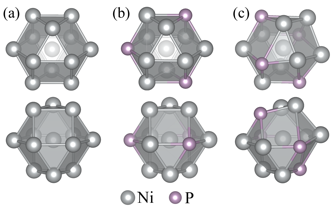
\includegraphics[width=0.5\textwidth]{str_ss}
	\caption{Coordination cube-octahedron around Ni atoms in fcc-Ni (a), Ni$_5$P-$P6_3/mcm$ (b), and Ni$_3$P-$Cmca$ (c) structures; upper row – view along three-fold axis, lower row – perpendicular to the three-fold axis
{\color{red}
-- У нас везде по тексту просто Ni$_5$P, а здесь он с пространственной группой. Нужно сделать единообразно, т.к. переходов по давлению нет, то пространственные группы можно не писать
} }\label{f:strs}
\end{figure}


Spin-polarized calculations show the presence of a magnetic moment in structures with a relatively high nickel content from Ni$_{14}$ to Ni$_8$P, as shown in Fig.~\ref{fgr:magmom}. 
In all other cases, the magnetic order is absent. The magnetic moment per nickel atom decreases with an increase in the specific phosphorus content in the system. 
With increasing pressure, the magnetic moment and magnetic ordering completely disappear at a pressure of 315, 360, 350, and 115 GPa for the Ni$_{14}$P, Ni$_{12}$P, Ni$_{10}$P, and Ni$_8$P lattices, respectively. 
Unlike the considered phosphides, the magnitude of the magnetic moment in pure nickel weakly depends on external pressure. 
With an increase in pressure from 100 to 200~GPa, the magnetic moment per nickel atom decreases from 0.58~$\mu_B$ to 0.5~$\mu_B$ and then remains practically unchanged.

\begin{figure}[h]
\centering
  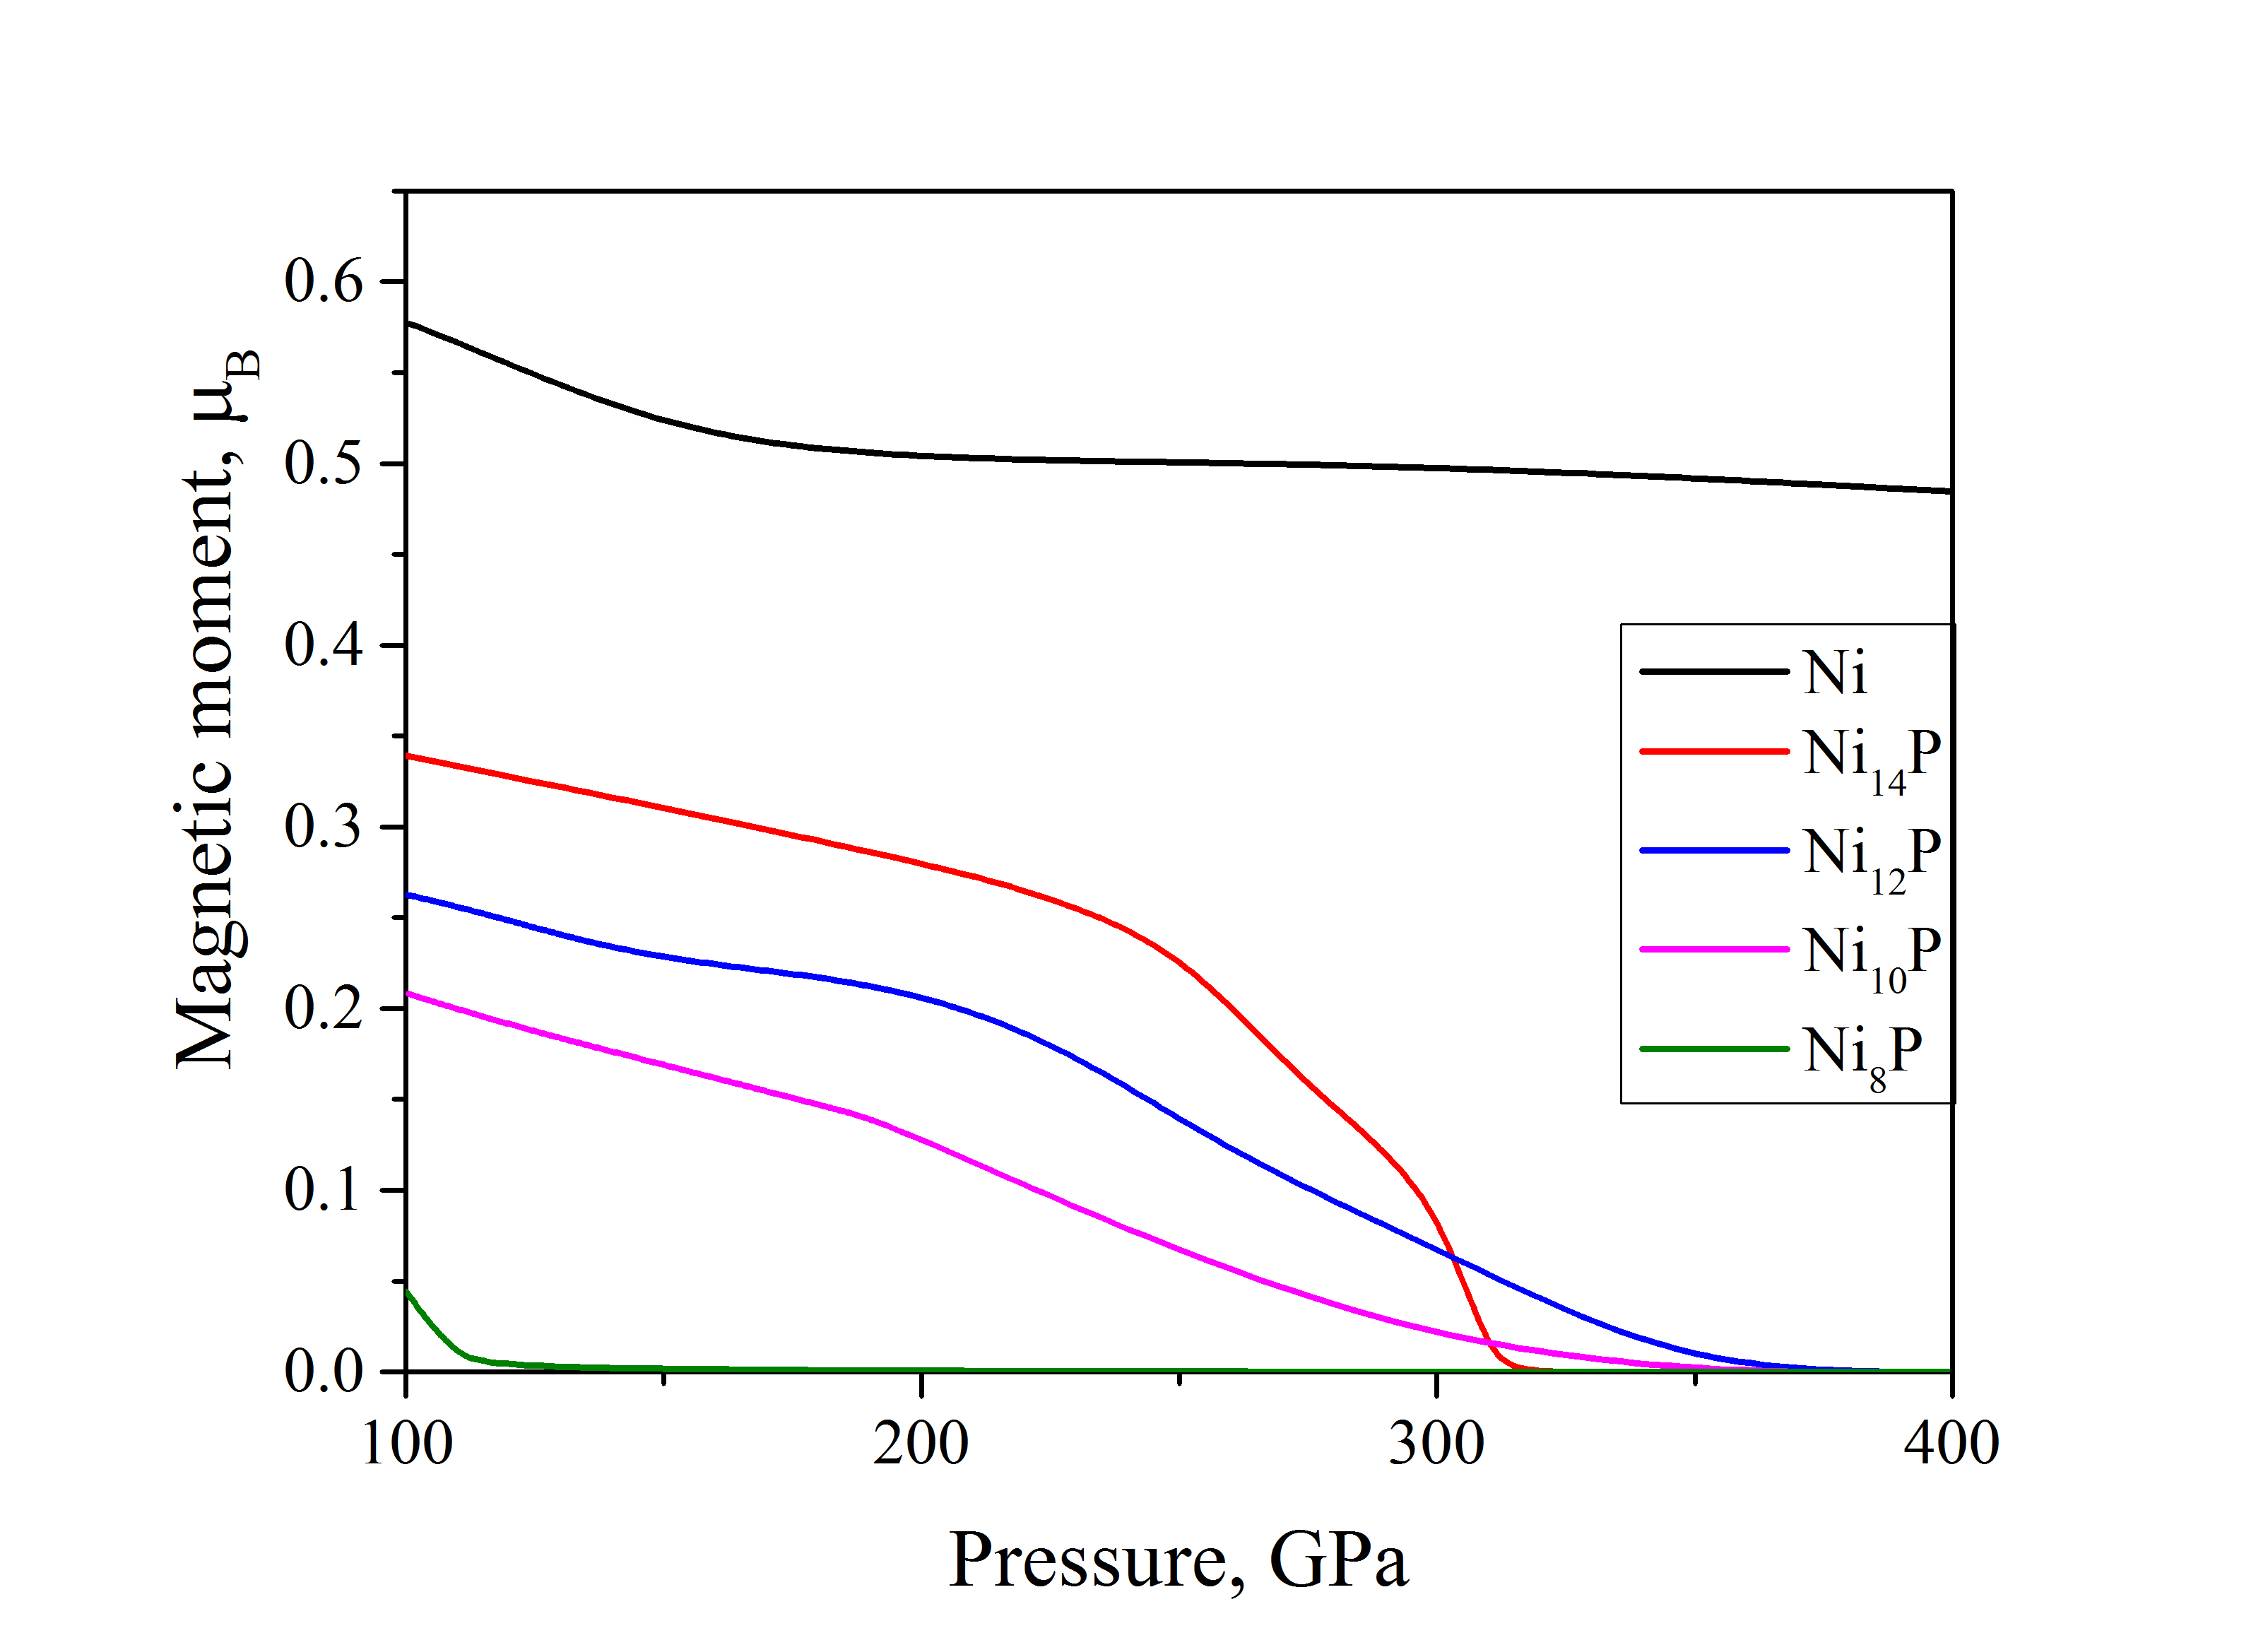
\includegraphics[width=0.45\textwidth]{magmom-uspex.jpg}
  \caption{Pressure dependence of magnetic moment (in Bohr magneton, $\mu_B$) per Ni atom for predicted Ni--P crystal structures.
  The dependence of the magnetic moment on pressure for pure nickel is given for comparison.
  }
  \label{fgr:magmom}
\end{figure}



%%%%%%%%%%
\subsection{Thermodynamic of Ni--P compounds}
%%%%%%%%%%

Both sets of the predicted and experimentally observed Ni--P binary compounds were used to evaluate the formation enthalpy $\Delta H$ with respect to the elemental solids Ni and P according to Eq.~\ref{Eq:enthalpy}, in order to explore the thermodynamic stability of Ni--P:  

\begin{equation}\label{Eq:enthalpy}
 \Delta H(\mathrm{Ni}_n\mathrm{P}_m) = \frac{H(\mathrm{Ni}_n\mathrm{P}_m)-nH(\mathrm{Ni})-mH(\mathrm{P})}{Z(n+m)},
\end{equation} 
where $H=U+PV$ is the enthalpy of each compound, $Z$ is a number of formula units in the unit cell of the structure and $\Delta H$ is the enthalpy of formation per formula unit. 
Herein, $U$, $P$, and $V$ are internal energy, pressure and volume, correspondingly. 
Detailed information about the element solids can be found in SI. Ссылка на рисунок.

The relative stabilities of the considered compositions at the selected pressures of 100, 200, 300, and 400 GPa, with $\Delta H$ evaluated per atom, are shown in the form of the co-called {\it convex hull} Fig.~\ref{fgr:convex_hull}, useful for assesing of the phases thermodynamic stability. 
Points corresponding to the phases with enthalpy lower than the enthalpy of mechanical mixture of the neighbouring compounds forms the convex hull on such a plot.
All points above the convex hull corresponds to the unstable phases, decomposing on the mixture of neighbouring compounds.
In addition to the predicted and described above Ni$_{14}$P, Ni$_{12}$P, Ni$_{10}$P, Ni$_8$P, Ni$_7$P, Ni$_5$P, Ni$_3$P, and Ni$_2$P structures, we have also considered Ni$_8$P$_3$ and NiP$_2$ structures, synthesised experimentally at ambient pressure \cite{}.

Predicted solid solutions Ni$_{14}$P -- Ni$_7$P are stable within all pressure range from 100 to 400~GPa, while solid solution enriched with phosphorus are stabilised with pressure.
Ni$_5$P became stable from  200~GPa and above, while Ni$_3$P from 300~GPa and above. Allabogdanite-Ni$_2$P is also stabilised against decomposition at 200~GPa.
Experimental phase Ni$_8$P$_3$ is stable in all pressure range, while NiP$_2$ destabilised above 300~GPa.

It has to be emphasized, that the results presented in Fig.\ref{fgr:convex_hull} are obtained neglecting thermal effects. 
In order to account for the effect of temperature on Gibbs energy, we use method of lattice dynamic.
Within this method, it is necessary to calculate the vibrational spectra of all the structures considered. 
We performed phonon mode calculations for all predicted structures, described above. 
Experimentally synthesised Ni$_8$P$_3$ was not considered in this context, due to the large size of the unit cell, containing 132 atoms.
Speculatively we assume thermodynamic instability of such a low symmetric structure in the filed of high temperatures, due to effect of entropy.

\begin{figure}[h]
 \centering
 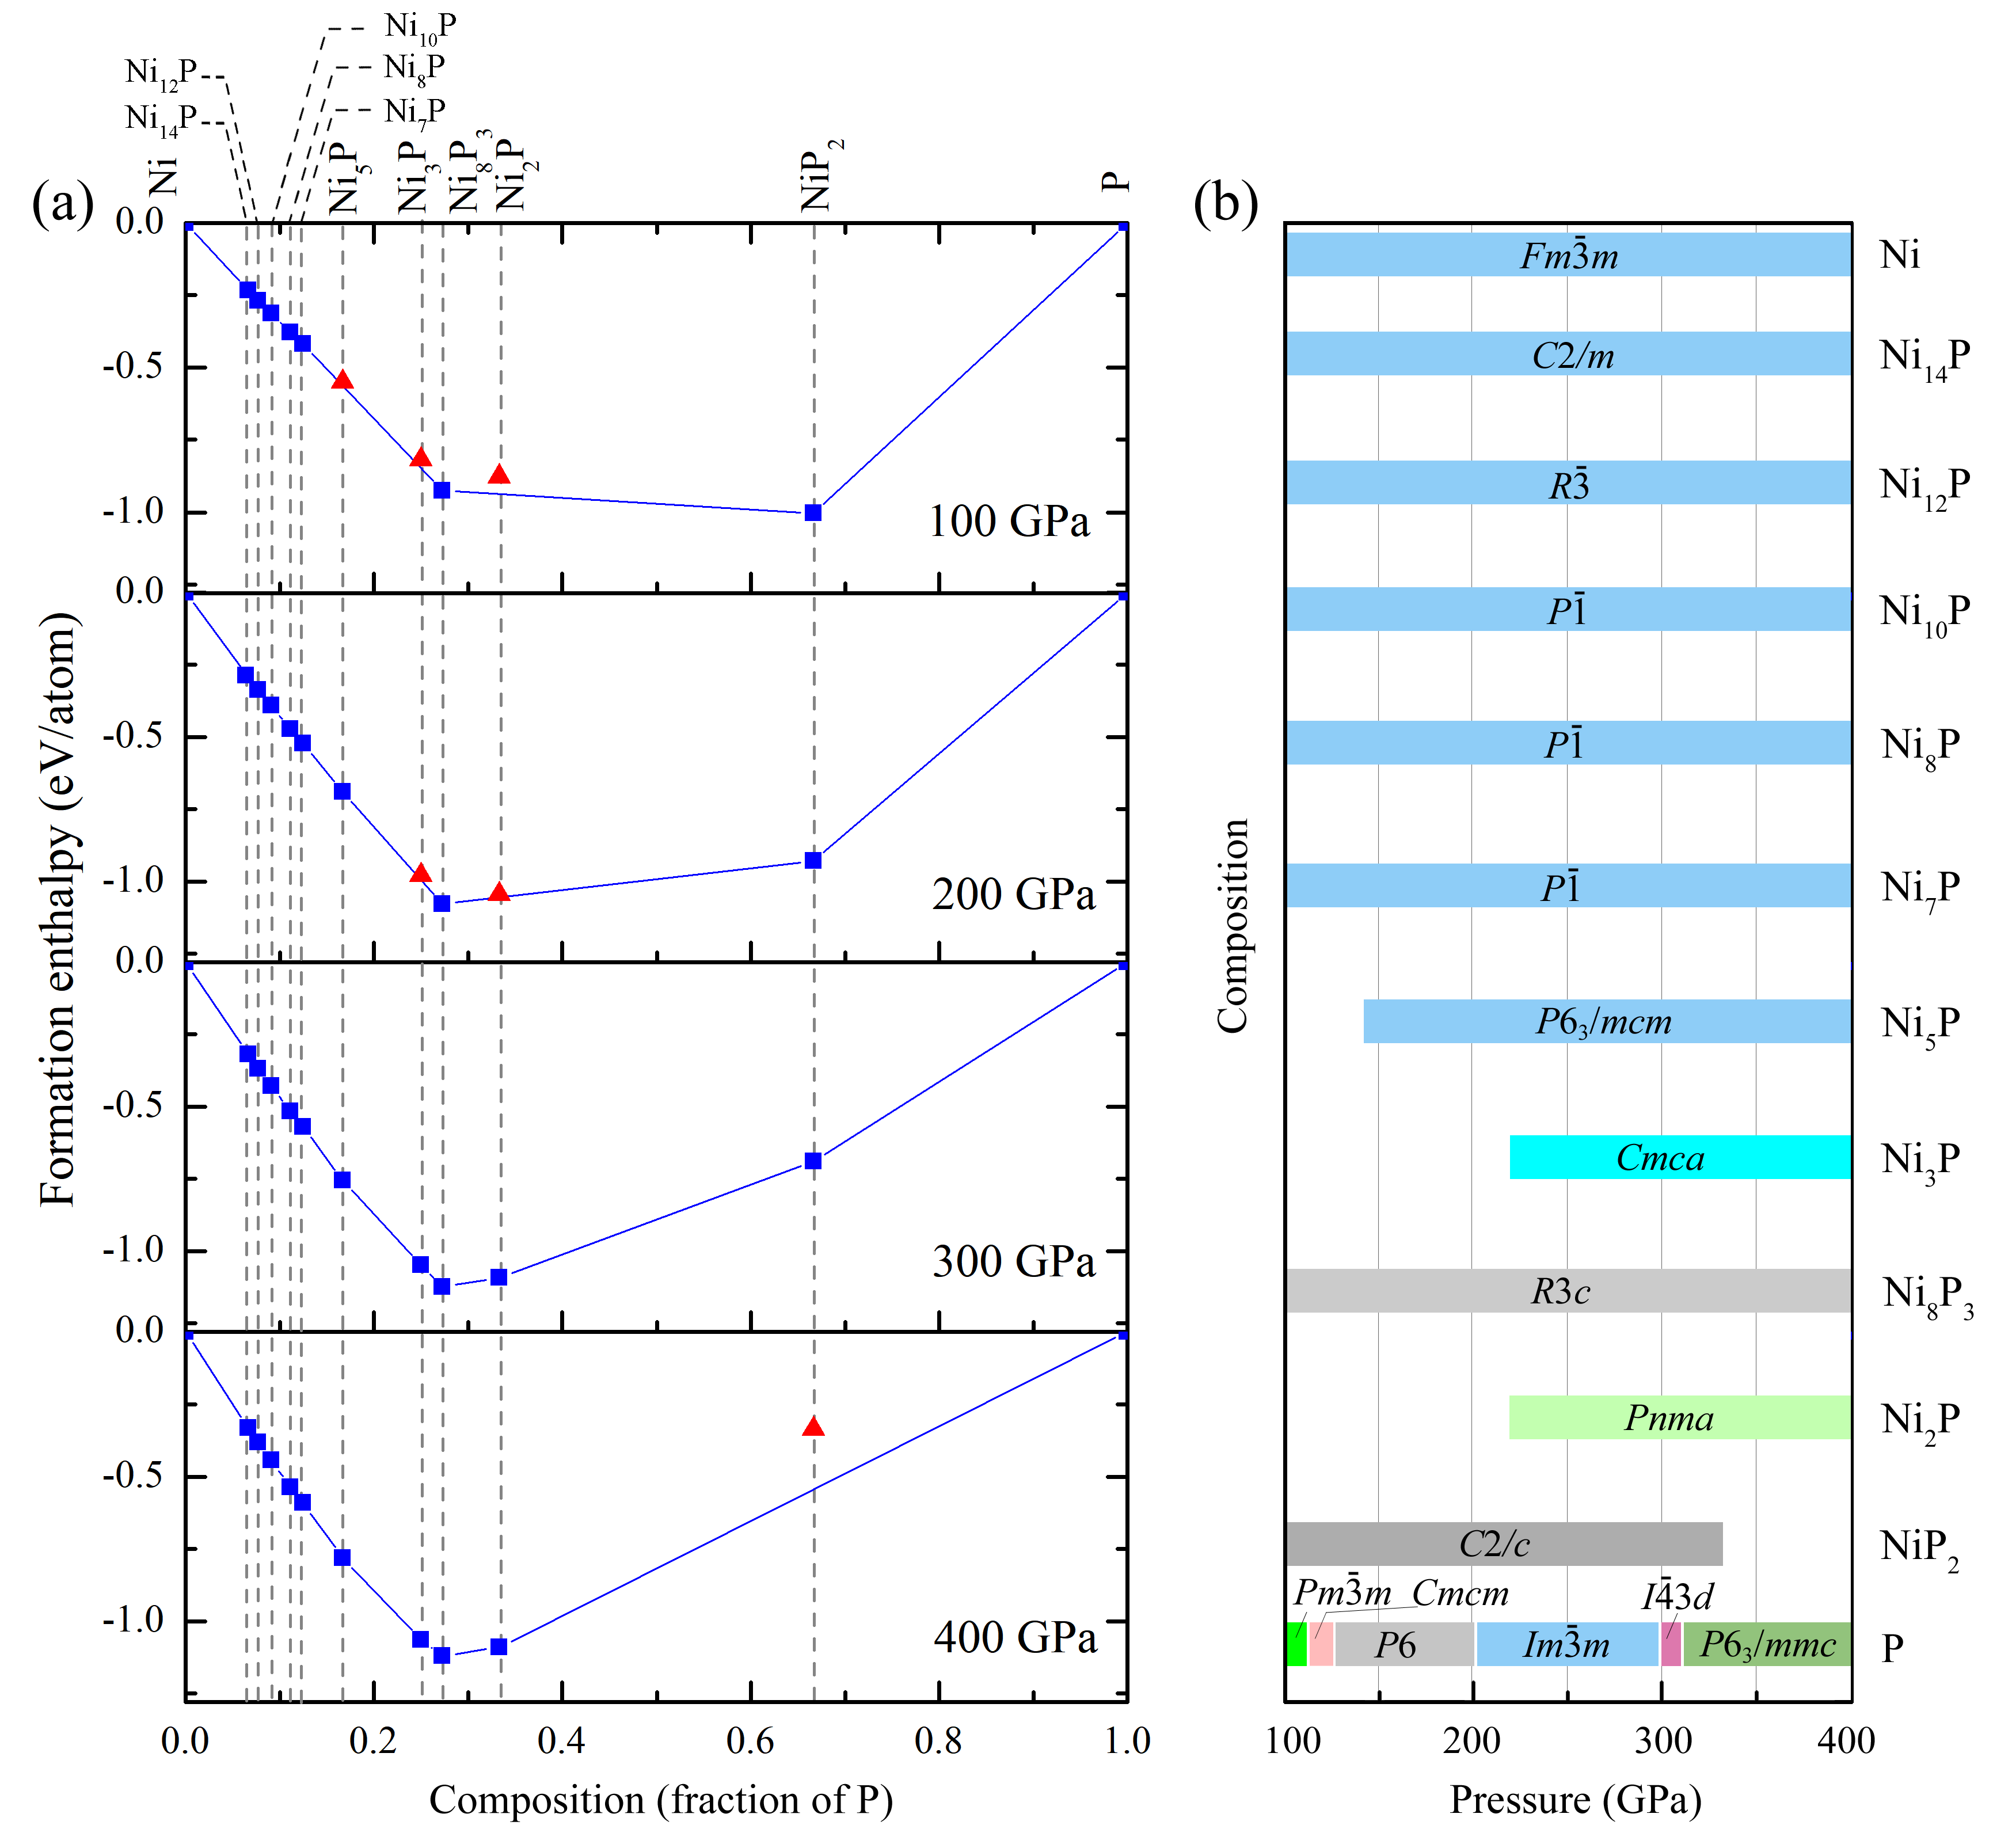
\includegraphics[width=0.45\textwidth]{convex_hull-2.png} %[height=6cm]
 \caption{Convex hulls of Ni--P system at various pressures and 0~K. Blue squares denote stable structures, red triangles - metastable ones}
 \label{fgr:convex_hull}
\end{figure}


\begin{figure}[h]
\centering
  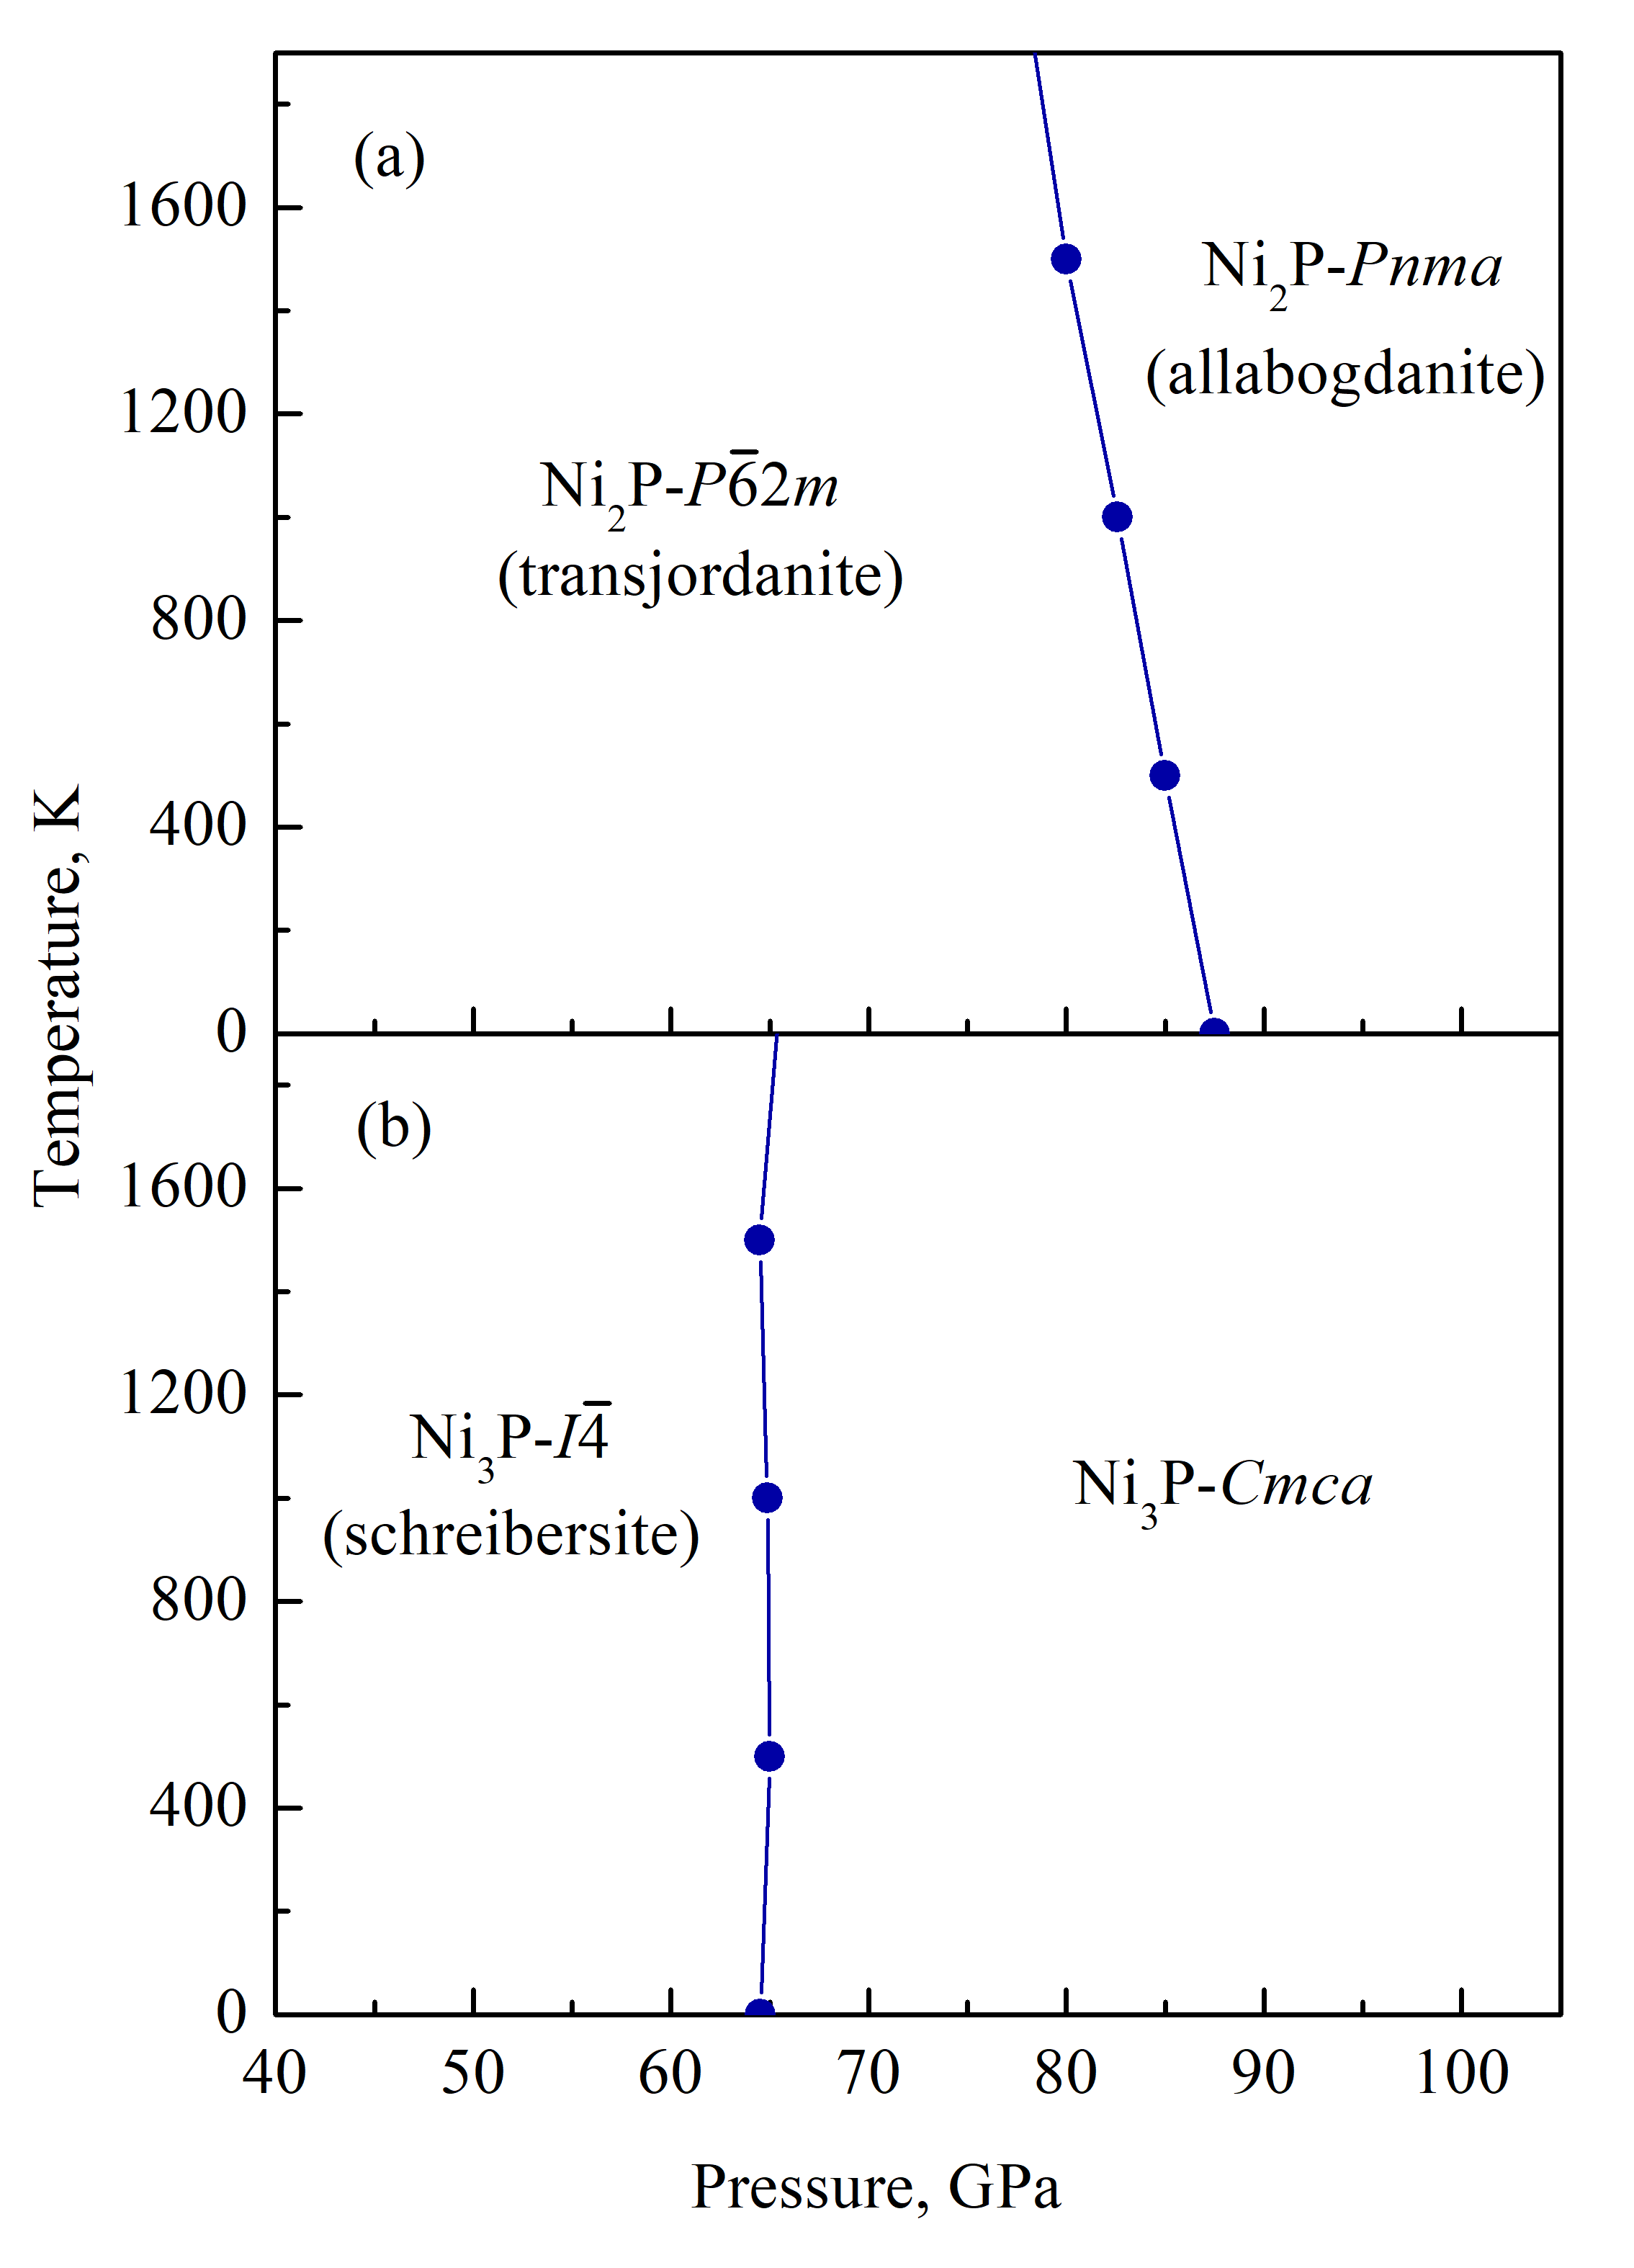
\includegraphics[width=0.45\textwidth]{pt_Ni2P_Ni3P.png}
  \caption{$P$-$T$ diagram of (a) Ni$_2$P and (b) Ni$_3$P}
  \label{fgr:PT-Ni2P-Ni3P}
\end{figure}

%\begin{figure}[h]
%\centering
%  \includegraphics[width=0.45\textwidth]{Ni3P_Phase_diagram.png}
%  \caption{PT-diagram of Ni$_3$P.}
%  \label{fgr:PT-Ni3P}
%\end{figure}

Due to natural ocurence of schreibersite-Ni$_3$P, allabogdanite-Ni$_2$P, and transjordanite-Ni$_2$P phases and their findings in metoritic rocks \cite{}, we determined PT phase diagrams for these compounds, presented in Fig.~\ref{fgr:PT-Ni2P-Ni3P}. 
The diagrams shows, that transition from barringerite to allabogdanite structure in the Ni$_2$P system occurs in the pressure range 77-88~GPa at temperatures 0-2000~K.
The transition from schreibersite to the found $Cmcm$ structure occurs at 62~GPa and pressure of phase transition is almost independent from temperature.


\section{Conclusions}
{\color{red}Я убрал этот раздел, точнее переместил его в аннотацию. В большинстве журналов он не обязательный, и я уже несколько раз видел рекомендацию "Раздел Выводы необходим только в том случае, если он содержит какую-то дополнительную информацию, не содержащуюся в аннотации". }

\section*{Acknowledgements}

The authors are thankful to the Center for Comput. Mater. Sci., Institute for Materials Research, Tohoku University and Novosibirsk Univesity Supercomputing Center for their continuous support of the supercomputing system to be used for our simulation works. 

The reported calculations on crystal structure prediction was funded by RFBR, project number 19-35-90043, calculations of PT diagrams – by the state assignment project of IGM, SBRAS.

\balance
%%%REFERENCES%%%
\bibliography{NiP} %You need to replace "rsc" on this line with the name of your .bib file
\bibliographystyle{rsc} %the RSC's .bst file

\end{document}



